
\chapter{Introduction}

\section{Context}

Robots were originally designed to assist or replace humans by performing repetitive
and/or dangerous tasks which humans usually prefer not to do, or are unable to do
because of physical limitations imposed by extreme environments. Those include the
limited accessibility of narrow, long pipes underground, anatomical locations in specific
minimally invasive surgery procedure, objects at the bottom of the sea, for example.
With the continuous developments in mechanics, sensing technology, intelligent control
and other modern technologies, robots have improved autonomy capabilities and are
more dexterous.

Nowadays, commercial and industrial robots are in widespread use with
lower long-term cost and greater accuracy and reliability, in the 2 fields like manufacturing,
assembly, packing, transport, surgery, earth and space exploration, etc.
Articulated robots, are among the most common robots used today. They look like a human arm and
that is why they are also called robotic arm or manipulator arm. In some contexts,
a robotic arm may also refer to a part of a more complex robot. A robotic arm can be
described as a chain of links that are moved by joints which are actuated by motors \cite{liu2021deep}.

The majority of robotics applications focus either on navigation aspects of mobile platforms
(e.g. industrial transportation systems, guide robots), or the manipulation of goods
with robotic arms (e.g., bin-picking applications). Nonetheless, few applications consider mobile manipulation
itself combining both robotic tasks. Despite there are several commercial mobile manipulators
in the market, there is a lack of real applications due to the complexity and uncertainty introduced
by combining both, manipulation and navigation \cite{liu2021deep}.

Due to the particular morphology of robotic arms, their scope is limited, and not all the positions of the
base near the table enable a successful picking. Traditionally, such mobile manipulation operations have
been solved using analytical planning and control methods. These methods require explicit programming of the
skills which can be very costly and error-prone particularly in problems where decision making is complex.
The performance of these models depends on how well the reality fits the assumptions made by the model.
Due to the impossibility of predicting all the cases that may occur in dynamic
and unstructured environments, these methods are generally impractical \cite{liu2021deep}.

Traditionally, well known planning and control methods have been widely used for scheduling
mobile manipulation behaviours, for example using the ROS navigation stack for navigation and SLAM
and MoveIt! for arm and object manipulation.

\section{Contribution}

todo: write contribution of the thesis work

\section{Structure}

todo: write structure: list chapters and their content briefly



\chapter{State of the Art and Literature Review}

This chapter will present the state of the art and literature review of the topics related to this project.
The topics are: Robotic Manipulator Control, Deep Reinforcement Learning in Robotic Manipulation and Mobile
Manipulation, Autonomous navigation, Object Detection and Grasping.

Particular focus is on the part regarding the Mobile Manipulation, since it is the main topic of this thesis
project. In particular, the potential challenges as well as possible benefits and disadvantages of using each
method will be discussed.

\section{Autonomous Navigation}

\section{Robotic Manipulator Control}

Currently, the control sequence of a robotic manipulator is mainly achieved by solving
inverse kinematic equations to move or position the end effector with respect to the
fixed frame of reference. Robots can be controlled in open-loop or with
an exteroceptive feedback. The \textbf{open-loop control} does not have external sensors or
environment sensing capability, but heavily relies on highly structured environments
that are very sensitively calibrated. Under this strategy, the robot arm performs by
following a series of positions in memory, and moving to them at various times in their
programming sequence. In some more advanced robotic systems, \textbf{exteroceptive feedback
	control} (closed loop system) is employed, through the use of monitoring sensors, force sensors,
even vision or depth sensors, that continually monitor the robot's axes or end-effector, and
associated components for position and velocity. The feedback is then compared to information
stored to update the actuator command so as to achieve the desired robot behavior. Either
auxiliary computers or embedded microprocessors are needed to perform interface with
these associated sensors and the required computational functions. These two traditional
control scenarios are both heavily dependent on hardware-based solutions \cite{liu2021deep}.

With the advancements in modern technologies in artificial intelligence, such as
deep learning, and recent developments in robotics and mechanics, both the research
and industrial communities have been seeking more software based control solutions
using low-cost sensors, which has less requirements for the operating environment and
calibration. The key is to make minimal but effective hardware choices and focus on robust
algorithms and software. Instead of hard-coding directions to coordinate all the joints,
the control policy could be obtained by learning and then be updated accordingly. \textbf{Deep
	Reinforcement Learning (DRL)} is among the most promising algorithms for this purpose
because no predefined training dataset is required, which ideally suits robotic manipulation
and control tasks. A reinforcement learning approach might use
input from a robotic arm experiment, with different sequences of movements, or input
from simulation models. Either type of dynamically generated experiential data can be
collected, and used to train a Deep Neural Network (DNN) by iteratively updating specific
policy parameters of a control policy network \cite{liu2021deep}.

Robotic control approaches can be broadly categorized into \textbf{model-based approaches}, such as
the ones using a Model Predictive Controller (MPC) and Inverse Kinematics (IK) computation,
and \textbf{model-agnostic approaches}, often characterized as \textbf{data-driven methods},
including Deep Reinforcement Learning (DRL) and other machine learning techniques.

\begin{itemize}
	\item \textbf{Model-based approaches} rely on explicit models of the robot's dynamics
	      or kinematics to formulate control strategies. MPC optimizes control inputs over a prediction
	      horizon based on the system's dynamics and constraints, while IK determines joint
	      configurations to achieve desired end-effector poses.
	\item \textbf{Model-agnostic approaches} learn control policies directly from data through
	      interactions with the environment. These data-driven methods leverage neural networks
	      to map observations to actions, allowing robots to adapt to complex and dynamic
	      scenarios without requiring an explicit model.
\end{itemize}

The main differences lie in the reliance on explicit models in model-based methods,
providing transparency and interpretability, versus the model-free nature of data-driven methods,
offering flexibility and adaptability to diverse and evolving environments.
Integrating these approaches can harness the strengths of both paradigms, combining the precision of
model-based control with the adaptability of data-driven learning for enhanced
robotic control capabilities in multiple scenarios and tasks.

An issue raised by the real-world application is the safety of the system while sharing
the workspace with human workers. Identifying and more importantly also certifying methods
how to collaborate with humans in the workspace in a safe way is
one of the key points for bringing autonomous mobile robots to real industrial applications.

The following paragraphs will describe the available methods used for robotic manipulator control.

\subsection{Mobile Manipulation}

Mobile manipulators that combine base mobility with the dexterity of an articulated
manipulator have gained popularity in numerous applications ranging from manufacturing
and infrastructure inspection to domestic service. Deployments span a range of interaction
tasks with the operational environment comprising minimal interaction tasks such as
inspection and complex interaction tasks such as logistics resupply and assembly. This flexibility,
offered by the redundancy, needs to be carefully orchestrated to realize enhanced
performance. Thus, advanced decision-support methodologies and frameworks are
crucial for successful mobile manipulation in (semi-) autonomous and teleoperation
contexts. Given the enormous scope of the literature, we restrict our attention to decision-support
frameworks specifically in the context of wheeled mobile manipulation. \cite{thakar2023survey}

As a quick aside, a disambiguation is necessary between the often interchangeably used
\textbf{"motion planning"} and \textbf{"path planning"}.
Although path planning only generates a path within the configuration space,
motion planning generates time-indexed motion trajectories. Instead much path-following only requires
spatial feasibility (e.g., obstacle avoidance), while motion planning
requires compatibility with spatiotemporal constraints (engendered in dynamics of both robot and
environment). It is also noteworthy that ultimately any path planning effort requires a final time
parameterization into a motion planning exercise before deployment \cite{thakar2023survey}.

The combined controllable degrees-of-freedom within the kinematic-chain (from both
mobile base and the articulated manipulator) presents the mobile
manipulator design architecture the opportunity to address very
complex tasks. However, resolving the redundancy (internal/external) is crucial to realizing
this potential. As the complexity of overall mobile manipulation process
increases, a two-stage hierarchical approach is often pursued:
\begin{enumerate}
	\item task planning/breakdown into a series of tractable motion planning
	      subtasks and their sequencing;
	\item motion planning of the high
	      degree-of-freedom mobile manipulator within each sequenced
	      task.
\end{enumerate}
It is noteworthy that the two steps (task planning and motion planning) are closely coupled
and should be solved concurrently but are addressed separately from a computational tractability
perspective \cite{thakar2023survey}.

However, a breakdown along the lines of mobile manipulator subsystems
(mobile base versus manipulator versus gripper or combinations)
or along the nature of the manipulation task (transportation versus grasping) feature prominently
in the literature. the task-level and motion-level planning frameworks
may be viewed as a form of "artificially constrained" motion planning within a higher dimensional space.

Although traditional methods have led to promising mobile manipulation skills in some specific tasks,
mobile manipulations tasks require the explicit programming of hard-to-engineer behaviours and often fail
in more complex tasks where the decision-making process is hard. In addition, such solutions
are generally very inflexible and error-prone due to the impossibility
of modelling all the uncertainty of dynamic industrial environments when those are programmed.

\begin{figure}[h]
	\centering
	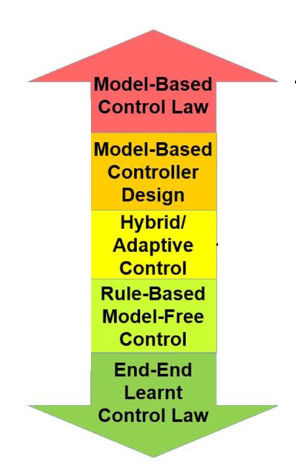
\includegraphics[width=0.2\textwidth]{img02.png}
	\captionsetup{width=0.6\linewidth}
	\caption{The continuum in the literature in regards to control
		methodology ranging from model-based to end-end data-driven
		control \cite{thakar2023survey}}
	\label{fig:img02}
\end{figure}



\subsection{Deep Reinforcement Learning - Data Driven Approach}

Explicit programming is often needed in practice to account for uncertainties in the environment and
sensors used, as well as to solve highly variable problems in an efficient way.
Explicit behavior programming is therefore often tedious and impractical, and more flexible solutions
are needed in environments where the robot must adapt to.
Alternatively, data-driven approaches address the main limitations of traditional methods and propose
to learn robotic behaviours from real experience, thus alleviating the cost of modelling complex behaviours.
This approach allows them to use deep neural networks to model the uncertainties of the environment,
which leads to a more robust controller compared to traditional ones.
Unlike deep learning (DL), the reinforcement learning (RL) paradigm allows to automatically obtain the
experience needed to learn robotic skills through trial-and-error and allows to learn complex decision-making
policies.

With RL, the explicit modelling of the problem is no longer required since the learnt models are grounded
in real experience. Recently, the combination of DL and RL, also known as Deep Reinforcement Learning (DRL),
has made it possible to tackle complex decision-making problems that were previously unfeasible. It combines
the ability of DL to model very high dimensional data with the ability of RL to model decision-making agents
through trial and error.
In fact, DRL has proven to be the state-of-the-art technology for learning complex
robotic behaviours through the interaction with the environment and solely guided
by a reward signal \cite{liu2021deep}.

While ML-based methods are generally used for offline forecasting, DRL is generally used online in
sequential decision-making problems. In fact, DRL allows to autonomously learn complex control policies
through trial and error and only guided by a reward signal. In the case of robotics, the most common
use case is to use such algorithms to model agents capable of performing continuous control of robots.

DRL has been successfully applied in a wide variety of areas such as robotics, computer vision and gaming.
Taking into account the difficulty of modelling complex decision-making robotic skills, DRL offers
a promising way to take advantage of the experience gathered interacting with the environment to
autonomously learn complex robotic behaviours. In particular, the field of DRL applied to robotics has
recently gained popularity due to the remarkable performance obtained in applications with high decision-making
and control complexity. Applications range from manipulation, to autonomous navigation and locomotion.
\cite{iriondo2023learning}

\begin{figure}[h]
	\centering
	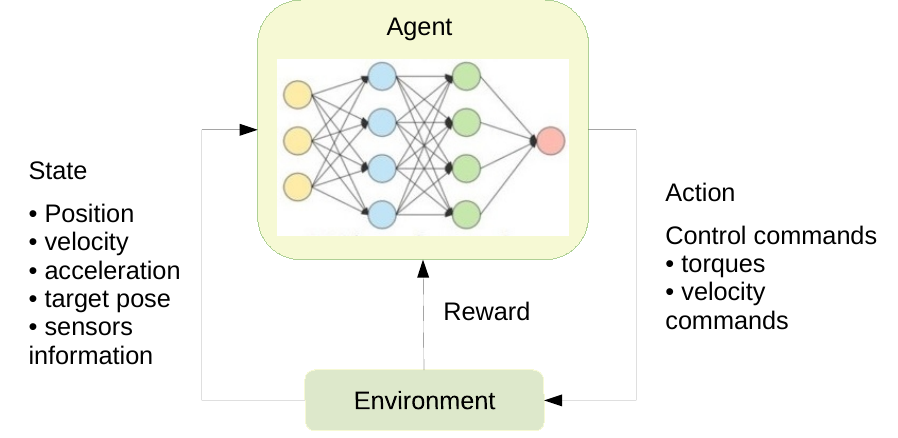
\includegraphics[width=0.7\textwidth]{img03.png}
	\captionsetup{width=0.8\linewidth}
	\caption{A schematic diagram example for robotic manipulation control
		using a data-driven approach such as DRL \cite{liu2021deep}}
	\label{fig:img03}
\end{figure}


\subsection{Challenges in Data-Driven approaches}

Two of the most important challenges here concern \textbf{sample efficiency and generalization}.
The goal of DRL in the context of robotic manipulation
control is to train a deep policy neural network, to detect the optimal
sequence of commands for accomplishing the task. The current state of the algorithm can include
the angles of joints of the manipulator, position of the end effector, and their derivative information,
like velocity and acceleration. The output of this policy network is an action indicating control
commands to be implemented to each actuator, such as torques or velocity commands. When the robotic manipulator
accomplishes a task, a positive reward will be generated. With these delayed and weak
signals, the algorithm is expected to find out the most successful control strategy for the
robotic manipulation \cite{liu2021deep}.

The challenges of learning robust and versatile manipulation skills
for robots with DRL are still far from being resolved satisfactorily for real-world application.
Currently, robotic manipulation control with DRL may be suited to fault tolerant
tasks, like picking up and placing objects, where a disaster will not be caused if the
operation fails occasionally. It is quite attractive in situations, where there is enough
variation that the explicit modeling algorithm does not work \cite{liu2021deep}.

However, even in this kind of applications, DRL-based methods are not widely
used in real-world robotic manipulation. The reasons are multiple, including sample efficiency and generation,
where more progress is still required, as both gathering experiences by interacting with
the environment and collecting expert demonstrations for imitation learning are expensive
procedures, especially in situations where robots are heavy, rigid and brittle, and it will
cost too much if the robot is damaged in exploration. Another very important issue is
\textbf{safety guarantee}. Not like simulation tasks, we need to be very careful that learning
algorithms are safe, reliable and predictable in real scenarios, especially if we move to
other applications that require safe and correct behaviors with high confidence, such as
surgery or household robots taking care of the elder or the disabled. There are also other
challenges including but not limited to the algorithm explainability, the learning speed,
high-performance computational equipment requirements. \cite{liu2021deep}


\begin{figure}[H]
	\centering
	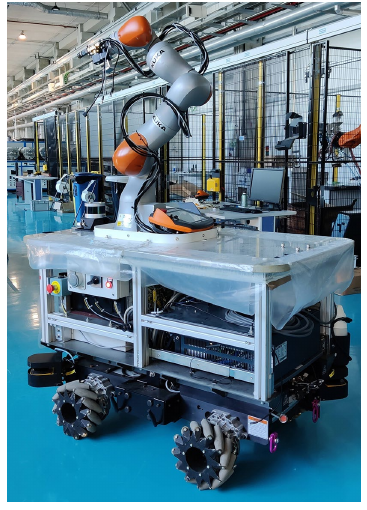
\includegraphics[width=0.5\textwidth]{img01.png}
	\captionsetup{width=0.6\linewidth}
	\caption{KUKA robot mounted on a mobile platform for pick and place tasks
		in industrial environments \cite{liu2021deep}}
	\label{fig:img01}
\end{figure}

\section{Whole-body mobile manipulator control}

In most control approaches to mobile manipulation, base and manipulator operation are strictly
separated such that at any given time only one primary control objective is
active. This separation principle is then augmented by a switching layer that determines the
currently pertinent control objectives. The advantage of such a control formulation lies in its
implicity, i.e., priorities can be separated among the arm and the base with individually
designed different control algorithms employed for each subsystem \cite{thakar2023survey}.

Instead, we refer to \textbf{whole-body control} as a unified control framework that considers
the mobile manipulator as a single system (arm manipulator mounted on a mobile wheeled / legged robot).
Despite the disadvantage that unified control needs to adhere to a single control framework,
it allows for the exploitation of mobile manipulation in the true sense of the term,
wherein the manipulator and mobile base can be controlled at the same time. This can lead
to several advantages during task achievement and makes the robot more dynamic in terms
of its capabilities. The formulation for this type of control involves considering
the onboard manipulator as an extended joint space of the mobile base, where the motion controller
considers both the base and manipulator state. As a result, base control can be completed
simultaneously without affecting much the performance of the end-effector manipulability
\cite{thakar2023survey}.


\begin{table}[H]
	\centering
	\begin{tabular}[c]{|m{3cm} || m{6cm} | m{6cm}|}
		\hline
		\raggedleft \textbf{Approach}                           &
		\textbf{Model-Based}                                    &
		\textbf{Data-Driven}
		\\
		\hline \hline

		\raggedleft \textbf{Control Strategies}                 &
		\customtablelist{
			\item Model Predictive Controllers (MPC)
			\item Whole-Body Inverse Kinematics (IK) Solver
		}                                                       &
		\customtablelist{
			\item Deep Reinforcement Learning (DRL)
			\item Imitation Learning
		}
		\\
		\hline

		\raggedleft \textbf{Features}                           &
		\customtablelist{
			\item Requires explicit modeling of system dynamics and kinematics
			\item Suitable for simple tasks, unsuitable for complex tasks
			\item Planning over end-effector pose or grasp in the workspace
		}                                                       &
		\customtablelist{
			\item No explicit modeling of system dynamics
			\item Learning from experience in simulation environments
			\item High-level planning over tasks, object detection, manipulation
			or other objectives
		}
		\\
		\hline

		\raggedleft \textbf{Interpret-ability and Adaptability} &
		\customtablelist{
			\item Explitic modeling implies high system interpretability
			\item Adaptable to many tasks but requires behaviors re-programming
		}                                                       &
		\customtablelist{
			\item Learned policies have very limited interpretability
			\item Learning from experience allows high adaptability,
			given proper GPU-parallelized training
		}                                                         \\
		\hline

		\raggedleft \textbf{Advantages}                         &
		\customtablelist{
			\item Small simulation-to-reality gap
			\item Adaptable to many tasks but with explicit programming
			\item No training required
		}                                                       &
		\customtablelist{
			\item No explicit modeling of system dynamics required
			\item Learning from experience allows high generalization
			\item Can perform well in unknown or dynamic environments
			\item Can provide high body-hand movement coordination
		}                                                         \\
		\hline

		\raggedleft \textbf{Disadvantages}                      &
		\customtablelist{
			\item Requires very accurate physical models for seamless integration
			\item Doesn't perform well in complex tasks or dynamic environments
			\item Difficult to adapt to complex tasks (low generalization)
			\item High computational cost for the solver in high DoF systems
		}                                                       &
		\customtablelist{
			\item Requires large amounts of training data and extensive training
			\item Very long time needed to fine tune the hyperparameters
			\item May result in unstable and jiggly movements
			\item May result in unsafe behaviors in real-world applications
			if not properly trained
			\item Suffers a lot from the simulation-to-reality gap
		}                                                         \\
		\hline
	\end{tabular}
	\caption{Summary of the main differences between model-based and data-driven approaches
		for robotic manipulator controls}
	\label{table:1}
\end{table}



\section{Object Detection and Grasping}

Grasp planning for mobile manipulators is a challenging problem that has been
dealt with in several ways in the literature. On the one hand, grasping requires coordination
within a very challenging high-dimensional constrained configuration space (mobile base /
manipulator / gripper). Further, grasping requires detecting object, constructing data-driven
representation, determining the gripper approach-vector, and computing all the mobile manipulator's
plans in the presence of uncertainty. Many of the traditional grasp planners (designed for stationary
manipulators) can be used for mobile manipulators once the mobile base has been fixed.
However, a generic grasping pipeline is desirable, which achieves arm-base-gripper
coordinated grasping given the information about object pose and
the operating environment. Such concurrent manipulator / mobile base motion approaches are being
explored till grasping is successful or at least until the gripper reaches the
objects (and only manipulator moves for grasping). This may not be optimal as grasping can happen
with the mobile base and the manipulator moving when the gripper is closing \cite{thakar2023survey}.


\TODO{review of different grasping methods, object semantic understanding via multiple views,
	object detection and pose estimation, grasping pipelines with heuristics, unknown objects}